\documentclass[12pt,a4paper,oneside]{report} 

%\documentclass[14pt,a5paper,oneside]{memoir}
%\setlrmarginsandblock{1cm}{1cm}{*}
%\setulmarginsandblock{2cm}{2cm}{*}
%\checkandfixthelayout

\usepackage[utf8]{inputenc} 
\usepackage{hyperref}
\usepackage{apacite}
\usepackage{cmap} 
\usepackage{url}
\usepackage[T1]{fontenc} 
\usepackage[osf]{libertine} 
\usepackage[scaled=0.90]{inconsolata}
%\PassOptionsToPackage{scaled=0.75}{beramono}
\usepackage[parfill]{parskip} 

\usepackage{listings}

\usepackage{graphicx}
\usepackage{float}
\usepackage{setspace}

\usepackage{tikz}
\usetikzlibrary{shapes,arrows,fit,backgrounds}
\onehalfspacing

%\usepackage[style=apa,backend=biber]{biblatex}
%\addbibresource{general.bib}



\title{Streams and currents:\\Wireless network sonification and other works} 
\author{Jonáš Gruska\\
Bachelor's Thesis\\
Institute of Sonology} 
\date{\today}

\begin{document}

\frenchspacing
\raggedbottom
\doublehyphendemerits=10000       % No consecutive line hyphens.
\brokenpenalty=10000              % No broken words across columns/pages.
\widowpenalty=9999                % Almost no widows at bottom of page.
\clubpenalty=9999                 % Almost no orphans at top of page.
\interfootnotelinepenalty=9999

\maketitle

\begin{abstract}
\end{abstract}
\clearpage
\setcounter{page}{3}


\chapter*{Acknowledgements}
I would like to thank my parents for supporting me during my studies. I would never be able to learn what I love without them. And of course, I would like to thank my mentor Paul Berg for his patience with my chaotic behavior and the whole Institute of Sonology for helping me to become who I want to be. Last, I would like to thank Janka Kobolková, Marko Uzunovski, Xavier De Wannemaeker, Maya Verlaak, Daniel Tóth, Peter Sych, Marek Chołoniewski and all my other friends in supporting me in my work, inspiring and pushing me forward.

\setcounter{tocdepth}{1}
\tableofcontents


\chapter{Introduction}

My work has never been turning around a single topic, yet there are connecting traits in all of it. \emph{Streams and Currents}, as in streams of data versus electric currents can be one of those traits. My passion for pure informational flow surrounding us in various forms is more than hinted in many of the topics I describe.

Sonification has grabbed my interest since my first experiments with programming computer music. By the time of my first contacts with the method, I was amazed by the possibilities presented by softwares such as Pure Data, where one could easily turn data-flows into their sonic representations. Using external streams as sources of inspiration seemed very rewarding, in terms of conceptual and practical realization. Not surprisingly, the method stick with me for some time.

This is the reason why I have chosen topics of sonification as a key element to my thesis --- it serves as one of the main inspirations to many of my works in various degrees. In next chapters, I will try to describe the context of my work with few significant examples and comparisons from the art world and the world of science, to give you a better idea where my ideas have started. My effort will also contain an attempt to distinguish two separate traits in approaches towards sonification, relevant for sonological context, and I will try to give an overview of devices which allow us to sonificate \textit{in situ}, the ones with scientific goal and those with purely aesthetic use.

After the topics of sonification, I will describe few of the most important projects I have worked on during years at Sonology (2009--2013), which should help to define my artistic approach in examples. This approach might not appear coherent at first, but one might notice that my work always shares specific qualities. Passion for technology, which is often present but not visible, love for sound as a pure physical vibration of the air and effort to turn invisible to audible.

This specific style of work is not something I have been developing consciously, one could say it came more from within. I am drawn towards technology since I was a child, spending endless hours in front of the flickering screens and lately in cloud of soldering fumes. But technology by itself does not satisfy me, I am trying to see beyond engineering, through the streams of electrons. Because my intrinsic power is sound. But I need bits and volts to reach it.

\chapter{Sonification and audification experiments}

\section{Thoughts on current state of sonification}

% What is this chapter gonna be about

Topic of sonification is intriguing for few reasons. Firstly, it benefits from interest of various groups of people --- scientists: biologists, mathematicians, creatives: musicians, sound artists and general public. Another is a belief, that this topic still has a lot of unrevealed potential. I will try to discuss this clash between scientific and artistic approach, various significant projects or artworks, as well as fields of opportunity blossoming from this duality.

% Sonification definition
Main understanding of the term \emph{sonification} is the \emph{``use of non-speech audio to convey information''}, or more precisely, it is the \emph{``transformation of data relations into perceived relations in an acoustic signal for the purposes of facilitating communication or interpretation''} \cite[p.~1]{Fitch}. These are definitions from probably the most relevant place to sonificication --- International Community for Auditory Display \cite{icad}, which organizes conferences and publishes books on the topic since 1992. Nicolas Collins puts it less formally, as a method for one to provide \emph{``aural alternatives to pie charts, line graphs and spreadsheets''} \cite[p.~7]{Collins2006}. All these quotations define it as an analytical, representative point of view, and the reasoning behind the use of the sonification in this sense is repositioning of the information from traditional semantic, visual or statistic level to sonic level giving ground to non-traditional data analysis via medium of sound or music. Interestingly, ICAD's first definition mentioning conveying \emph{information} rather than data can also give an understanding that sonification is not only about data patterns; and whether we try to sonify weather forecast, biological systems or our emotions is not important --- they are all qualified.

I believe the analytical approach towards sonification is rather clear and well defined. Books such as Sonification Handbook \cite{Hermann2011} prove that ICAD and its fellow researchers have done exquisite work in examining of the topic from various points, resulting in apparatus allowing us, artists to built upon. Although arts and sciences have many things in common, it happens so that aesthetic approaches toward sonification projects are in my opinion quite different.

%Some scientists residing on the analytical side are concerned with addition of music grammar and finesse, because it might get in the way of the data representation, \emph{``the music would be another language to learn''} \cite{Vickers2006}.

% Division proposal
That is why I would like to propose a division in this definition. There is one part of sonification world, described above --- that is, an analytical, `auditory display' world. My proposition adds \emph{an artistic world}, where the main goal of the process is not to make certain data accessible for aural analysis, but rather to use those data as a essence of specific aesthetics. That means, one is no more looking for a scientific tool, but on a sonic instrument, source of inspiration and compositional data. It might as well be described as a matter of aim behind the use of sonification methods in his work: whether works are aimed to inform a listener or provide him an auditory display of some data, or the sonification is used for its characteristic aesthetics.

Use of streams of data for compositional and sound generating purposes is very familiar to electro-acoustic composers, artists and performers. Sonification in artistic view is pushing the idea little further --- instead of algorithms, \emph{real world} data are used, although reaching their exact, understandable representation becomes additional or even insignificant, rather than essential. It might be, that there is deeper meaning behind the selection of the data stream (when artist sees the action as political act), so it is important that the point I am describing is more theoretical --- real works are more often combining certain degree of aesthetics with conveying information through sound.
%Benefits of sonification\\
%- pattern substraction\\
%- abilitity to filter in frequency domain\\
%- ability to focus on details in various distances\\
%\\
%\cite{Hermann2011} page 3

%Reduced listening vs. Causal listening\\
%\cite{Vickers2006} page 2

%SNIPPETS:\\*

To give some real world examples, I would like to point out few significant works which use sonification as its main concept or method, and while doing so, I will try to exercise my proposal for the new sonification definition division.

One of the most classic examples of sonification is \emph{Geiger} (or \emph{Geiger–Müller}) \emph{counter}, particle detector measuring ionizing radiation. This tool is known for its direct connection between environmental value (in this case it is radiation) and sound, it is one of the most known sonification tools. Technically, method of auditory display of the information is use of pulses --- representations of electrical charges (and consequential discharges) of the inert gas in the Geiger–Müller tube caused by particles or photons of the radiation. Higher amount of electrical discharges (being higher amount of audio pulses coming from speakers) is signaling greater density of particles of the radiation, thus higher radiation in the environment \cite{Knoll2010}. Geiger counter is clearly a \emph{analytic} sonification tool, with its main purpose being representation of certain information, rather than using the information as an artistic basis.

I have chosen Geiger counter for another reason than simply being ideal representation of scientific and analytic attitude towards sonification. It is also a standalone and portable instrument. This opens up a possibility for its artistic use, even though its design is serving purely for research purposes. As I suggest later on in subsection discussing my wireless sonification project, I find interest in portable sonification tools for various environmental experiments. These tools can be used as an immediate instruments, serving artists with unconventional musical experience of the data \emph{in situ}.  

Geiger counter can be also viewed as representation of sub-method of sonification, \emph{audification}. To quote Sonification Handbook,  \emph{``audification is a technique of making sense of data by interpreting any kind of one-dimensional signal (or of a two-dimensional signal-like data set) as amplitude over time and playing it back on a loudspeaker for the purpose of listening.''} \cite[p.~301]{audif}

Audification is sonification simplified to the most basic level. Majority of the common real-time sonifications are then audifications as well, e.g.\ listening to the whale songs or bat echolocation, where the only transformations which happen on the data are changes of the playback speed.

One of the most interesting sonification works is work of Christina Kubisch \cite{ChKubisch2012}. I have chosen her as an icon of electromagnetic induction a method, even though there is a wider spectrum of artists using the same tools. She generally appears as the icon of the method, so it will not be different in my thesis. Kubisch is German sound artist born in 1948. She studied classical instruments such as flute and piano, but have later turned to studying electronics at Technical Institute of Milan. Since than she has created various sound installations, usually combining electronics and delicate sounds. In a work I would like to mention --- Electrical Walks, Kubisch is focusing on audification of electromagnetic fields with the use of induction coils, headphone amplifiers and headphones. This works as a nice example of artistic audification, where the purpose seems to be in finding of interesting sounds within the world of electromagnetic fields rather than scientific analysis. 

Induction coils are acting as antennas and natural amplifiers, which when in right setting, can provide excellent tools for electromagnetic sensing. Alternating current (AC) oscillations of the electromagnetic field are inducted on the coil, thusly creating AC signal. This AC signal is than amplified and can be directly treated with any audio devices as sound. It is an oscillation, similar to signal produced by oscillators.

I have designed a simple pocket amplifier for this purposes called \textbf{Eletrosluch} (see fig.  ~\ref{fig:elektrosluch}). This device provides 100x gain for the coils and it is powerful enough to drive headphones. Its main benefit is the size and portability, ideal for an electromagnetic sonic explorations. The version 1.0 (on the ~\ref{fig:elektrosluch}) used tape head which I have extracted from an old tape player as the induction coil. Amplifying circuit was based around LM386 amplifier, which I have replaced in v1.1 with low-noise operational amplifier TL071. Tape heads have been replaced with \emph{pick-up coils}, which were in previous century, while attached with its suction cup to telephone headset, used for noise-less recordings of telephone calls. 

\begin{figure}  
  \centering
    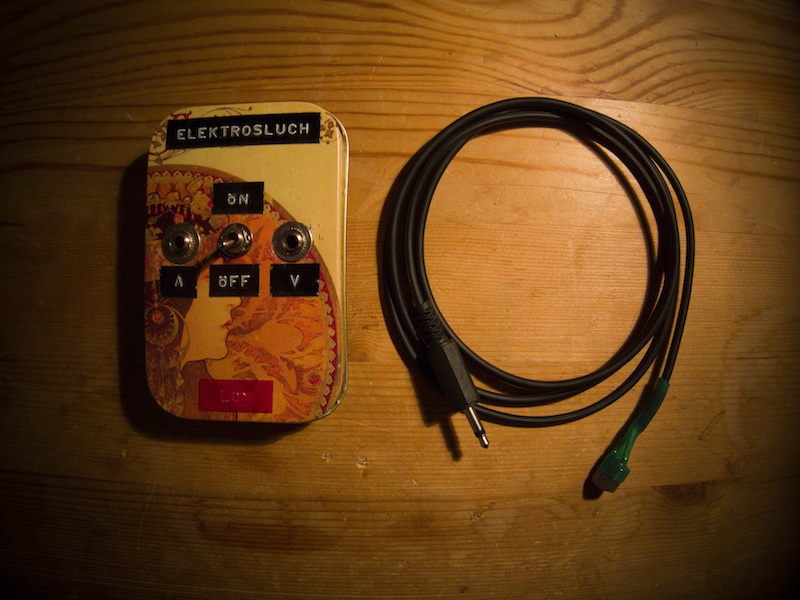
\includegraphics[width=0.9\textwidth]{img/elektrosluch}
	\caption{Elektrosluch 1.0}
	\label{fig:elektrosluch}
\end{figure}

Probably closest to my network sonificiation work is the one by Michael Chinen  and Shintaro Miyazaki's Institute for Algorhytmics. 

Michael Takezo Chinen is an American programer. He studied computer science and composition at University of Washington, Tokyo Denki University and Dartmouth College with Richard Karpen, Charles Dodge and Naotoshi Osaka. He was part of the developers of popular open source audio editing software Audacity. His artistic focus resides in software sonification, in sense of a method as in sense of a target. Prove to this claim are his works \textbf{lstn} and \textbf{FuckingWebBrowser}, which I will now try to examine in greater detail. \cite{mchinen}

Both \emph{lstn} and \emph{FuckingWebBrowser} are based around sonification of computer based streams and data. To be more precise, lstn is \emph{``a program that sonifies real-time debugging data of other programs''} and FuckingWebBrowser is \emph{``simple mac web browser with memory sonification based on WebKit''} \cite{Chinen2010, Chinen2010a}.

These works are quite similar to my work Sonodump\footnote{More information about Sonodump can be found in 2.2 Wireless sonification}. For example, as well as Chinen in FuckingWebBrowser, I also deal with browsing of the internet as with the initial trigger and data stream for the sound generation. One might find it as analogous action to e\.g.\, bowing of a violin. Address bar becomes a bow and stream of data (conscious decisions about URLs to type in the address bar) is the angle and pressure of the bow on the strings. 

Chinen makes an excellent point for artistic stand towards sonification. Aim towards translating real information towards listener is missing (maybe only to a very experienced one); use of sonification plays a different, artistic, role, rather than the one of auditory display. It is about using a pure source of data for sound generation, not a source of information meant to be mediated towards audience.

His work is representative and direct, yet its main point is not to convey information. Auditory display becomes `useless' from scientific or research point of view and becomes interesting as an artwork for its specific aesthetics.

Chinen's work has been strongly connected to Institute for Algorhytmics, led by Shintaro Miyazaki. He is a post-doctoral researcher at Humboldt University in Berlin dealing with \emph{``epistemology, archeology, history and theory of everyday technologies, which store, transmit and process informations and their dynamic relation to sound, rhythms and other sorts of time-varying signals.''} \cite{Miyazaki2012}. From his projects, I want to point out his collaboration with Martin Howse \cite{howse} called \textbf{Detektors}.

Detektors is \emph{``an open, collaborative project which uses sonic strategies and DIY-devices to make audible the hidden infoscapes of our time. The present website will show data, recordings and cartographies of different spectral ecologies and trans-sonic machinic agencements.''} \cite{detektors}. Website of the project contains many sound recordings of the electromagnetic fields (audifications) from radio-frequency range as well as cartographic information about such sources. It is a study of the electromagnetic pollution, sonic behavior of digital devices in the context of a geolocational sound recordings.

\begin{figure}  
  \centering
    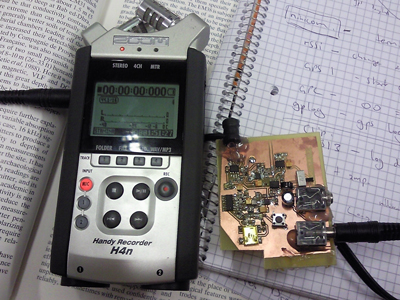
\includegraphics[width=0.9\textwidth]{img/detektor}
	\caption{Detektors ``Detektor'' device}
	\label{fig:detektor}
\end{figure}

For `detection', specially designed device is used as seen on figure ~\ref{fig:detektor}. Core of the hardware is logarithmic detector chip AD8313 produced by Analog Devices. This chip takes AC signals from up to 2.5 GHz  (upper border most used wireless network range is 2.4 Ghz \cite{802} and demodulates them into audible sphere. This is somehow similar to work of Kubisch, but there is a difference in the frequency spectrum target. Method using induction coils leaves us only with electromagnetic AC signal within our hearing range and within the limitations of the amplifying system, but method using demodulator allows us to listen to high frequency communication, such as bluetooth and wireless radio. Interestingly, Detektors and Kubisch's work both share emphasis on placing of their sonic discoveries within cartographic space.

These works have proven to be very effective in their directivity and immediacy. One can just simply turn on the device and listen to `invisible' streams of data, constantly present and surrounding, yet unnoticed by our senses. 

My wireless network sonification work is strongly related to that concept. My passion for revealing omnipresent data streams, penetrating our tissues on daily basis is possibly very similar to what has driven Kubisch or Miyazaki to build their own sonification systems.  

%Sonification of objects using distance sensors.
But before I jump to describing my works, I want to mention one more example of sonification project: a project of Gil Weinberg called \emph{BrainWaves}. It is based on interactive auditory research of electrical stimuli applied to \emph{in vitro} neuron cultures. I picked this work for the inherent collision of scientific and artistic approach.

To briefly describe the project, \emph{BrainWaves} is \emph{``sonification installation that allows a group of players to interact with an auditory display of neural activity. The system is designed to represent electrical spike propagation in a neuron culture through sound propagation in space. Participants can simulate neural spikes by using a set of specially designed controllers, experimenting and sonically investigating the electrical activity of the brain.''} \cite[p.~9]{Weinberg2006}. The particular part which caught my interest is desire to experiment with the subject of sonification interactively. Classic idea of stream of data is missing --- instead of discrete information there is a system, which needs to be sonified. As a comparison, one can imagine hitting an oil barrel in a goal of exploring its acoustic properties --- physical model, where system becomes the subject.

Since main subject of the auditory display is propagation pattern simulation, the authors have decided to use spatialization as key element of representation. As they argue against visual display, \emph{``sonification can be more effective than visualization in such a spatial application because the human auditory system is able to perceive synchronous spatial stimuli from every point within a space, while visual perception is limited to physical range of sight.''} \cite[p.~9]{Weinberg2006}. For the purpose, 8 speakers in space are used to provide sufficient clues for the exact propagation pattern.

For the interactive standpoint, custom made drum trigger instruments were created using piezo elements to represent electrical spikes in the system. Performers are asked to hit these in specific way --- after first propagation ends, performer placed closest to its ending is bound to start another one, by hitting his own instrument. At this point one could see an interesting connection between \emph{sonification} and \emph{gamification} as a very close methods of bringing data streams and system under closer, possibly more understandable, examination.

As authors conclude, the method of using almost only spatialization for auditory display purposes was not completely successful, since they noticed that part of performers was using visual representation of the process (provided during event) to orient in the process rather than simply \emph{listen} to the positioning. 

From the analysis stand point, I see this work as bordering between scientific and artistic approach. The effort to analyze real scientific system combined with use of almost musical methods and instruments seems as an interesting way of reaching sonologicaly relevant results. It appears that authors have not seen scientific results as a pure purpose of the work. Using (musical) instruments, focus on aesthetics of the sound themselves both suggest this was not classical scientific approach.

Hopefully, at this point I have presented sufficient amount of various works which allow me to prove my point in making distinction in methods or approaches in sonification. I personally believe, that it is important to recognize artistic sonification as specific subject, since I have not found this disambiguation to be done sufficiently.

\section{Wireless network sonification}

As a part of my own experimentation with untraditional sources for musical or generally sonic data I decided to extend my line of work on the layer of wireless networks. Project I would like to describe in this chapter is dealing with wireless network sonification as a main artistic source for sonic performance and installation. In basic terms, it catches data streams `from the air' and transforms them directly into sound using set of tools and methods. This work has been presented as a performance and an installation. In case of performance, I have used the live coding technique to change the aspects of the sonification. This was done via purposeful tampering of the networks by creating artificial data streams as well as by modifying the parameters of sonification.

\subsection{Work process and technical details}

To describe the process in higher detail, I would like to define some basic terms of the technical side of the project first, and then continue by describing my point of view on an even more important artistic side.

% Describe the whole concept in general first
% As musician using a metal box for performance
% Ffffucking web browser
I will start with packets and packet analyzers, since they are key elements of my wireless network sonification efforts. Packets, and in this case \emph{network packets} are units of formatted data. It is basically a standard of packing predefined amount of information into understandable format, easily and efficiently transmittable over networks. \emph{Packet analyzers} or \emph{sniffers} are tools for silent interception of network traffic. In technical terms, it is software (or hardware) which passively receives all data link layer frames passing through the device’s network adapter, not just those directed towards recipient. They are generally used by hackers, while also having legitimate use by system and network administrators or security experts. Sniffing is possible due to the physical characteristic of network. Either with LAN (Local Area Network) or unencrypted WLAN (Wireless LAN), all data passing through the system are accessible to everyone. It is than a job of WLAN or LAN adapters (network cards) on the site of client to separate its part of the data using filtering based on MAC (Media Access Control) address. MAC address is an unique identifier of every computer's network adapter. Except simple network MAC filtering, it can be, e.g.\, also used for assigning IP address by ARP (Address Resolution Protocol) and DHCP (Dynamic Host Configuration Protocol).

By enabling the functionality of network device called \emph{promiscuous mode}, one is able to avoid this filtering and obtain all present network packets. This is possible as well as for wired as for wireless adapters, thus for wired or wireless networks. Of course, there are certain limits to this. For example when a \emph{network switch} is placed in the network, it is not possible to receive everything. Network switch, different from \emph{repeater} or \emph{hub} (device only physically `multiplying' the cable), is more advanced device and acts as a MAC filter by itself, therefore working as a network filter by itself. \cite{Pallavi2012}

A classic example of a sniffer is \textbf{tcpdump}. Tcpdump was developed at University of California in 1987 by Van Jacobson, Craig Leres and Steven McCanne and its main use is traffic analysis. Unix Manual entry describes it as ``dump traffic on a network'' \cite{tcpdump}, but that is very reducing. Over the years since its first release it has become a rather complex and powerful tool. One of the features of tcpdump is that it can work easily with both LAN or WLAN packets (and actually many other obscure network protocols) and therefore provides us with various data sources for our artistic purposes. Because of its enormous functionality on one hand and lightweight operation on other, it has become my favorite tool for wireless network sonification and will be discussed more, later on in the text.

In the beginning of my research I was considering few options, ways, and processes. I was motivated to learn C programming related to audio, so that became my first choice. It has started by writing my own sniffer, based on library developed by same developers as the ones of tcpdump. This library is called \textbf{libpcap} (PCAP stands for Packet CAPture) and serves for implementation of tcpdump functionality to one's software. Obviously, this was not very easy task to do, especially for unexperienced C programmer as myself. After I finally managed to sniff data using my software, the next step was to use \textbf{PortAudio} library to implement the audio part of the project.

Finally I partly succeeded, by writing \emph{Sonodump}. Sonodump worked closely to what I wanted --- it \emph{sniffed} the network data and reflected current traffic via sound. The conversion was done through treating data harvested from the network as audio data --- simple WAV file. User had only two options to select from: which interface should be used (wireless or wired) and what sample rate is expected. Use of the term sample rate is a bit inaccurate, because there is no correct, real sample rate of the stream --- it is not audio stream. We can just guess or purposefully select some value to affect the way the sonification behaves. Lower sample rates resulted in a rather low-frequency based sonic content and higher settings create more higher frequencies. This occurs simply because of the speed the network data are read. It can be described as an obscure case of wavetable synthesis with tables generated by the network stream.

Sonodump already gave some interesting results, yet it was not very efficient. My programming skills were not just on the right level to optimize the code properly. Therefore I needed to look for other options. In autumn 2011 I was asked by organizer of AudioArt festival in Krakow, Marek Chołoniewski to present my sonification work on his festival. I happily agreed and immediately thought of wireless sonification project. But Sonodump was not enough in this case --- I needed something more flexible, powerful and in the end, more interesting.

One of the questions was whether to treat the sonification process in a more traditional way, lacking interaction with the stream which is being sonified. I felt inner conflict between keeping certain level of purity and working on the most successful and pleasant aesthetic experience. In the end, the idea of live interaction with the stream of data won, with argument planning for achieving non-traditional way of control over the resulting sound. With image of this wild, partly unpredictable instrument I started to research other, new technical solutions.

As mentioned before, Sonodump was not optimal and had few problems (in programmers lingo --- bugs), but after some time, I discovered other very useful set of commands present on Linux systems.

Main motivation for work with Linux / UNIX was availability of all the tools I required (sniffer, network tamperer, raw data stream player) and system shell, terminal. This shell allows me to do scripting (basically programming with advanced tools) and very importantly for this project, \emph{pipelining} and \emph{redirecting} --- interconnecting processes and files. For example, output of one a process can be streamed in real time to an another without user caring about any `middle-man' text file or thinking about memory allocation. This comes in particularly handy, when one wants to \emph{sonify} something. 

Good example is redirecting of a non-audio file to the sound card. What this represents is treating the file as a stream of data consequently feeded to the sound card as it would be audio data --- coming for example from a mp3 player. On some Linux distributions (Linux comes in various flavors) it is enough to write this command to the terminal:
\begin{quotation}
	\texttt{\textbf{\$} cat SONIFY\_ME.txt > /dev/dsp} 
\end{quotation}

Command \texttt{cat} reads the file \texttt{SONIFY\_ME.txt} --- which is a regular text file; and by using the symbol \texttt{>}, bash takes care of writing it to \texttt{/dev/dsp} --- which is a virtual port for sound card. Writing to this port opens a stream on the sound card and plays given data as audio.

%In my definition, a sound or piece of music can be called composition even though it is not composed by a composer.
This is very primitive and direct method of sonifiying any data and sometimes results in quite surprising compositions. It is not an easy task to determine whether this primitive mode of sonification can be called composing and who actually is a composer in the system. Is it me, the person which conceptually combines data stream and their sonic interpretation or is it the program which actually decides on the translation of the data to sounds? I believe that the result of sonification of a non-audio data file can be seen as a composition, but I am not completely sure who is the composer in that situation. I am generally inclined to the idea, that the program, data file and my concept are composing in \emph{symbiosis} of the Machine, Data and the Human.

I was particularly charmed by the sound of archive containing source codes of tcpdump itself. The song (or a file --- in this sense it is almost synonymous) offers range of gestures which are composed in a unexpectedly pleasing way. There are even appearances of few rhythmic patterns and primitive melodies. To give you a clear image, I have linked a recording of this composition in \autoref{appendix:a}.

Basic process of reading network data and converting them directly to sound is not much harder. The \texttt{cat} command is now replaced with \texttt(tcpdump), which is a tool mentioned before --- traffic analyzer, \emph{sniffer}.
\begin{quotation}
	\texttt{\textbf{\$} tcpdump -i wlan0 -A > /dev/dsp} 
\end{quotation}

Tcpdump opens a packet capture process at a device \texttt{wlan0} (wireless module). Option \texttt{-A} represents conversion of the captured data to ASCII symbols, allowing us to always read them in the terminal as text. These are than again, streamed into \texttt{/dev/dsp} which serves as the sonifying module. This already gives us some amount of sonification of the network with just single line of code. 

Next step was, to think about what other ways are there to experiment with. One of the options was change of the sample rate of the /dev/dsp (sound card) on-the-fly and thus change of the resulting sound as with the Sonodump. After some research on the topic it seemed as rather complicated and bulky approach, so I had to think of some other method. That was when I discovered \textbf{aplay}, part of ALSA. ALSA is amongst OSS and Jack one of sound systems used for audio on Linux. The most important function of aplay for me was the possibility to read data from pipeline (i.e.\ from other process) and to modify few parameters of the reading. Great addition was fact, that it is easy to have almost unlimited amount of aplays playing at the same time, even from one source. ALSA is handling the mixing of the streams to the sound card.

Interaction (or as some people call it --- tampering) with data stream was, as I mentioned earlier, not an easy decision. There was part of me trying to preserve the original streams in their pure form, but in the end, I have decided to work with streams as with a live instrument. Of course, the control is not as direct as hitting the drum. My \emph{stick}, which I use to hit the system, is hidden in the terminal. 

\begin{figure}  
  \centering
    \tikzstyle{block} = [rectangle, draw, 
	    text width=6em, text centered, minimum height=2.8em, node distance=4.5cm, scale=0.8, top color=white, bottom color=black!10, rounded corners=2pt]
	\tikzstyle{line} = [draw, -triangle 90, scale=1.2]


	\begin{tikzpicture}[node distance = 2cm, auto]
	    % Place nodes
		\node [block] (nds) {Network data stream};
		\node [block, above of=nds, node distance=3cm] (rni) {Router, other network users};
		\node [block, right of=nds] (sniffer) {\textbf{tcpdump} \\Packet sniffer};
		\node [block, right of=sniffer] (aplay) {\textbf{aplay} \\ Actual sonification};
		\node [block, below of=sniffer] (me) {Me \\(Performer)};
		\node [block, right of=aplay] (aout) {Audio output};

		% Draw edges
		\path [line] (rni) -- (nds);
		\path [line] (nds) -- (sniffer);
		\path [line] (sniffer) -- (aplay);
		\path [line] (aplay) -- (aout);
		\path [line, rounded corners=5pt] (me) -| node [near end, above, scale=.8, rotate=90] {Arbitrary data} (nds);
		\path [line, rounded corners=5pt] (me) -| node [near end, below, scale=.8, rotate=90] {\begin{tabular}{l}
		Sonification\\ parameters 
		\end{tabular}} (aplay);

		\begin{scope}[on background layer]
		    \node[fill=lightgray!50,inner sep = 4mm,fit=(aplay)(sniffer),label=above:Computer] {}; 
		\end{scope}

	\end{tikzpicture}
	\caption{Data flow of Sonodump performance}
	\label{fig:wifisonifi}
\end{figure}

From technical view, I was mainly generating arbitrary traffic using set of tools created by hackers (penetration testers in everyday job) dedicated to stress testing of networks. Creating such artificial loads is useful for few reasons: one being recording a reaction of routers to such massive amounts of data and the other one (a bit more evil one) is a bit more complex. When router crashes because of an overload, all users on the network must reconnect. And reconnecting means resending passwords as well, so it creates ideal situation for sniffing of the sensitive data.

My use was obviously less malicious, I was experimenting with the behaviors of the sonic output under various kinds of attacks. To get a good overview over the whole process, see ~\ref{fig:wifisonifi}. I have sketched the basic concepts of the different aspects of the system, which should help you to understand flow of information and the consequent transformation to audible domain.

At this point I have had prepared a sufficient toolkit for my upcoming performance and installation, therefore I started to focus on the artistic aspects, nuances of the work.

\subsection{Performance and Installation}
I have performed only once with this setup. As mentioned, it was on AudioArt festival in Kraków and it has been successful, for few various reasons. My initial approach was to try to create some kind of static object in space, which would than perform \emph{for me}, as in --- instead of me. I would be sitting away from the device with laptop in my lap and I would control the process from there, over network. This has been the idea until around 4 days before the performance, when after talking with my friend I have decided to twist my plan in quite radical fashion and do a live welding of my instalation during the performance.

To elaborate a bit more, I have always been intrigued by welding and the atmosphere it establishes. Extremely, harmfully bright lights, bursts of current through metals, high voltage buzz. Sonically, sound world of welding machine was actually quite matching to sound world of my wireless sonification software. But that was not the only reason behind the use of such different instrument. From the beginning, I aimed to build specific kind of a sculpture, and 4 days before the performance, it still was not ready. Plan for the object was to create a pyramid from metallic rods, which would serve as representation of antenna, \textit{prism for streams}. Therfore, it clicked, and I decided to built one, during the performance, with the use of the welding machine.

\begin{figure}  
  \centering
    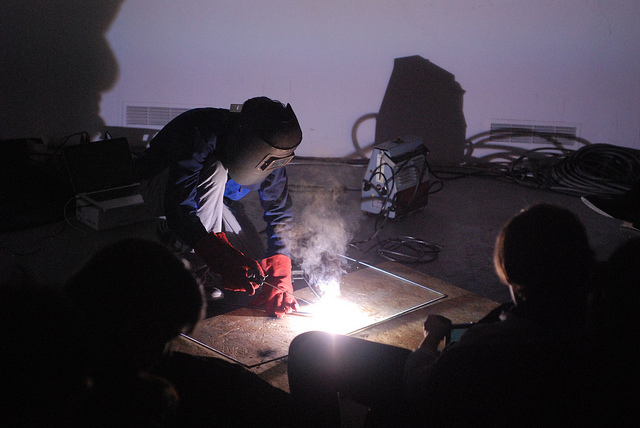
\includegraphics[width=0.9\textwidth]{img/zvarac}
	\caption{Sonodump performance}
	\label{fig:zvarac}
\end{figure}

I was not an experienced welder at all, I have welded only two times in my life before the performance. This was supposed to scare me, but it only drove me further --- I acquired all the necessary protection, such as special welding protection helmet and gloves, and started to experiment. It was the day before the performance. Interesting note might be, that the venue had to change their circuit breakers in the power grid for higher current draws, all because of my performance.

During the performance, welding did a terrific job on creating two things. First being the already mentioned atmosphere --- smell of hot metals, crackling and sizzling of the electric current were simply wonderful and spectacular. When I talked to the people from the audience after the performance, many have mentioned the connection to the welding happening `on the streets'. Everyone has few experiences with welders and the bright light of the process, which actually connects to the second aspect I managed to create. 

That was the fact, that since I used dangerous amounts of light (welding light can burn parts of the lenses), people have closed their eyes. While performing, I was of course focused on the performance itself, but when I saw video from the event, I noticed that most of the audience has either closed eyes or their heads are turned to the ground. Many faces just reflected pure focus on the sound. This was of course an amazing effect, which I actually did not expect to happen in first place. Since I was basically forcing people to look away, they really did and listened.

The installation was continuing in similar manner as a performance. By using \textbf{bash}, shell scripting language, I was able to create various simulations of myself. I programmed a simple robot, which was starting attacks on the local network, the same way as I would. This allowed me to create installation which was interesting enough and could have been presented in place for longer period of time without my attention.

Unfortunately, I have ran into problems with the installation during weekend, since gallery owners were turning their routers off for that period (since no one was working in offices). Therefore, wireless sonification did not work for few hours, since there was no network to be sonified. Fortunately I managed to provide my own router and setup my own network in place shortly.

\subsection{Future}
I am still intrigued by the network sonification, and I am at the moment working on a new projects these days. One is recreation of Sonodump called \textit{Hlysnan}, designed to be more user friendly application for Mac OS X and Linux. Aim of this application is to give visual feedback to people (displaying of the raw data streams), as well as live control of the sniffing and sonificating parameters via graphical user interface of the software. Project is still in its alpha stage. For the core of the software, I have migrated to C++ with use of OpenFrameworks framework for interface development.

Second project is not realized yet, but connects my idea of wireless sonification to handheld devices (as mentioned earlier). With use of affordable computers such as Raspberry Pi, I want to create pocket device which would than allow one to simply walk around and \emph{listen to networks} in a mobile way. So far I have it working as easily deployable small box for quick sonifications, but it would be nice to have physical interface for the interaction with the sonification and the sniffing process.

\begin{figure}  
  \centering
    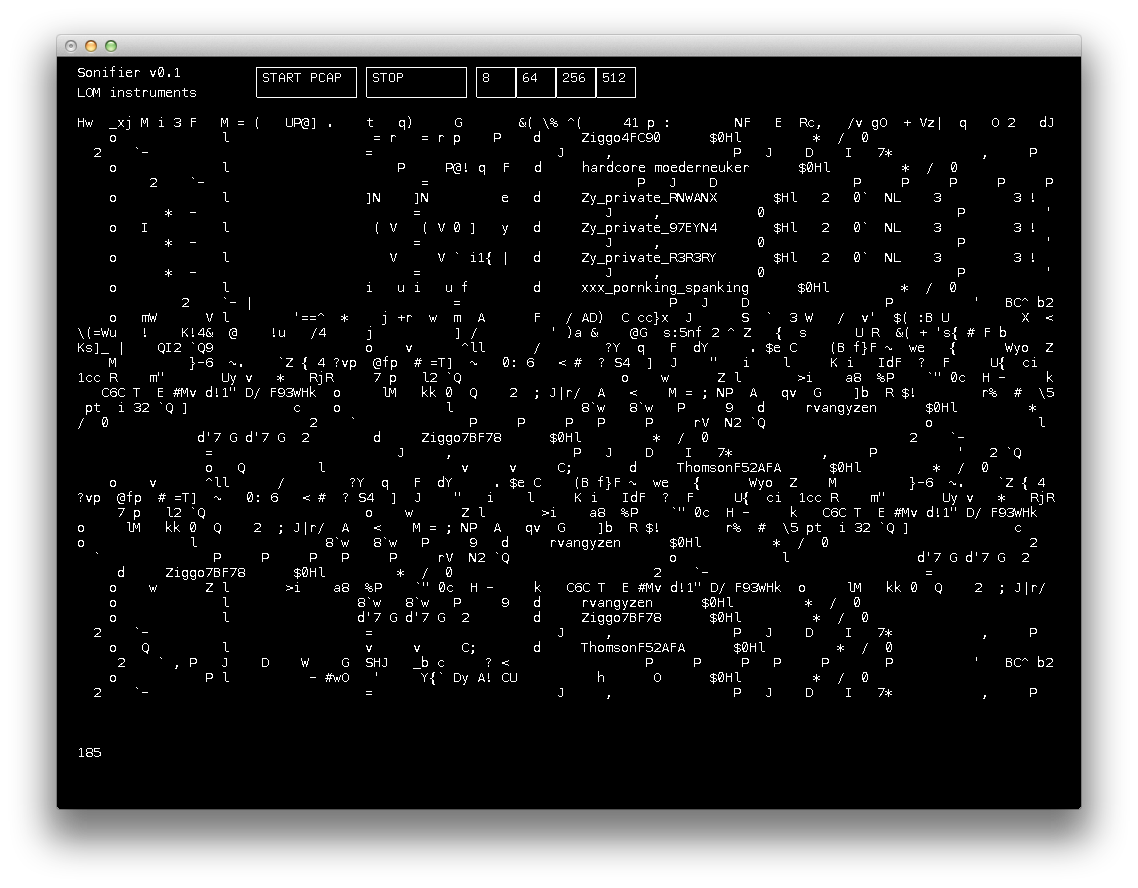
\includegraphics[width=0.8\textwidth]{img/hlysnan}%
	\caption{Hlysnan v0.1 --- reinventing the sonodump}
	\label{fig:hlysnan}
\end{figure}

\clearpage

\section{City attributes sonification}

City attributes sonification is an project I have been confronted with in 2011 in Czech Republic. At the time, I have been invited to lead a workshop on topics dealing with sound, city and architecture. Event was a part of bigger festival dedicated to city of Brno (second biggest city in the country).

Organizers have happily accepted my proposal for the exact topic, being sonification of the city. I was very curious to see what will people possibly come up with and it actually turned out rather nicely. Workshop lasted 4 days. In the beginning I have introduced the basic concepts of sonification and audification, presented few significant (yet varying) works in the field and commenced brainstorming.

Workshop resulted in few interesting ideas. One of the most inspiring one was the one of Lucie Vítková. Lucie actually studied at Royal Conservatory for a year after the workshop. Her idea was to do direct live interpretation of the street.  In the beginning, we have split the street into sections and each of us was responsible for sonification of his part. Each of us had different instrument and different set of rules. Sonification worked via visual clues, which we (as musicians) interpreted into sounds / music. Visual clues could have been anything happening on the street --- trams, walkers or wind. One of us decided to sonify a person walking on the street by simulating the rhythm of his footsteps on a small home-build synthesizer.

Another project, by Václav Peloušek, was based on my research of wireless sonification. He has harvested (or `sniffed') portions of data from surroundings of our workshop space and sonified them in rather unusual way. He has used online services which allow one to read out given text and he fed them the raw wireless data, containing plenty of humanly unreadable data. He used service which offers czech (in sense of pronunciation) voice, allowing to have amusing pronunciation of these noisy characters in a sequence. Last project to mention was one of Peter Gonda, which used open source software \textbf{driftnet} to work on a visual level. Driftnet allows one to sniff wireless network and directly parse images in the streams. This means, that whenever is one opening a certain image on a network, we were able to see the image directly on the screen.

I have as well realized a project I had in mind for some time, that being timetable sonification. Timetables are quite accurate in reflecting certain rhythms of city. They are carefully adjusted for the needs of citizens to allow smooth and on-time distribution, especially in peak hours. This results in various frequencies of arrivals of transport, depending on the time of the day. For this purposes, I have constructed a Max patch called ``Šalina samohrajka'' (šalina means tram in slang of Brno). Than I harvested few different timetables of trams in Brno and fed them to the patch to create a score (see fig. ~\ref{fig:salina}).

\begin{figure}  
  \centering
    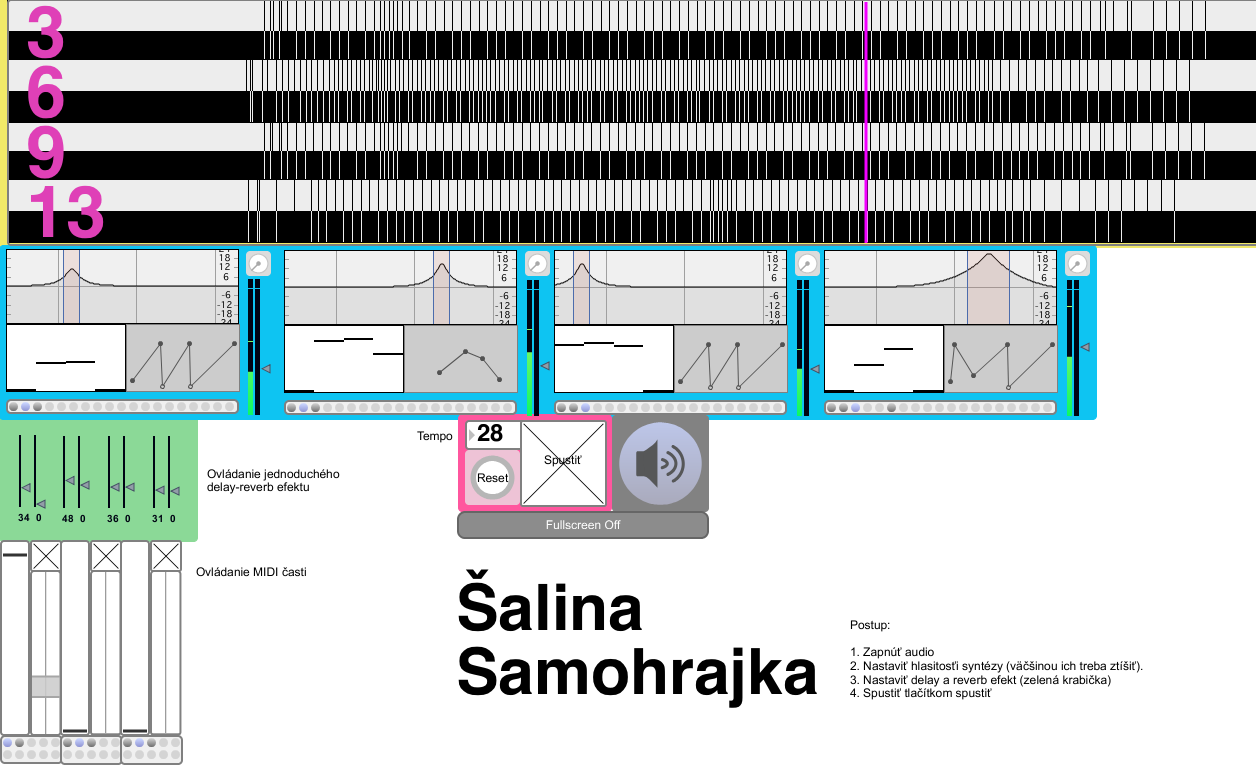
\includegraphics[width=0.9\textwidth]{img/salina}
	\caption{Šalina Samohrajka --- timetable sonification Max patch}
	\label{fig:salina}
\end{figure}

Each of the scores (tram lines) was binary grid. This means, it had 1440 fields (for every minute in a day) and field where no tram arrived was 0, and the one with arriving 1. These scores served as triggers for my percussive synthesizer, built in the patch. I have decided to work with percussive sounds, since my aim was to represent certain kind of rhythm of the city, its `breathing'. On the final day of the workshop, I have (amongst others participating) performed with this patch. I have mainly controlled the synthesis and playback time (the speed of the day) to create various situations and perceptual differences of time in the city. 

Whole project was rather interesting experience, unfortunately I was not able to motivate everyone to do solid work. Few people had natural fear of computers and did not really understood the concepts, which was of course problematic. But for the ideas such as the one of Lucie, I know it was worth doing.

\begin{figure}  
  \centering
    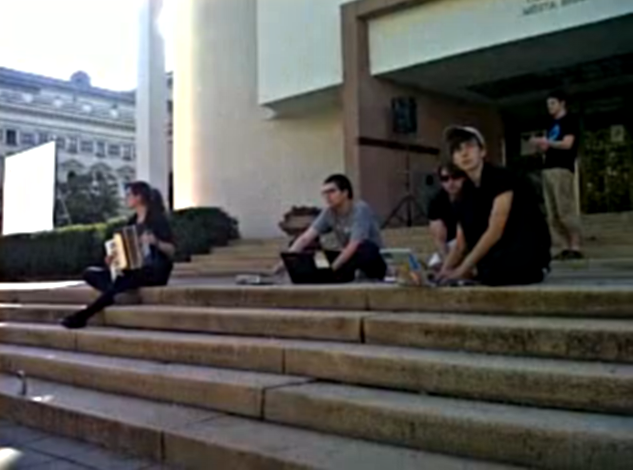
\includegraphics[width=0.9\textwidth]{img/workshop}
	\caption{Street sonification project in front of House of Arts in Brno}
	\label{fig:workshop}
\end{figure}

%\chapter{Modularity and physical instruments}
%\section{Reinvention of the physical musical environment}
%\section{Musical use of microcontrollers and low-level computers}
\chapter{Other works} 
\section{Binmatu} Binmatu is an audiovisual drone performance I have been executing during last two years.

\subsection{Introduction} I have never been very extensive listener of drone music and I could hardly relate to most of the works I have heard. The idea of extremely slow movements didn't please me aesthetically nor technically. At the time, I preferred wild improvisations with high pace of changes and especially high variety of sonic content.

This has changed when I have ran into works by Phill Niblock and La Monte Young. I realized, that drone music needs its own time to be perceived properly. One could say it needs to induce some kind of a trance state, where person becomes hypnotized by the simplicity of the composition and sound. At that point, the subtle changes start to make sense and whole world of microscopic compositions and performances starts to occur. Our ears (and brain) finally start to focus on details, which as under magnifying glass, have liberty to become big movement, filled with spine-chilling realizations.

In particular, I was heavily impressed by Phill Niblock's work, 22 minute long \emph{A Trombone Piece}, for trombone and tape machine, which works as a looper. There are possibly just 2 or 3 notes played (within interval of a second) during the whole work, yet it creates astoundingly heavy and dense atmosphere. Nothing really happens, just short breaks of the player for inhaling before upcoming blow. Sonologists may hear comb filtering occurring on overlaying trombone signals and frequency beating. Our perception, missing the regular level of stimulation starts to work differently and becomes more sensitive to slight details. My listening changes over the whole duration of the piece, from the regular alert position of a listener to meditative and contemplated state of mind. 

\subsection{Starting point} My work started at the point of musical hibernation in some sense. I was at that moment doing artistic residency at OKNO medialab in Brussels, dealing with my project of designing open source modular gardening system. Most of the day surrounded by soldering iron, electronic components and working on the code. I was not communicating with many people during the day and my only companion was a computer (and social contacts accessible through it). It was a strange mental state, where I experienced many hours of silence and loneliness. I feel it is important to describe these conditions, because I believe they are very much reflected in the resulting work. 

I started composing one night. For me as sonologist, composing often means writing code. To elaborate, after four years at Institute of Sonology, I sometimes see myself as composer which have exchange five line staff with (five) lines of code --- writing algorithms is writing music. And that is what I was doing, writing line after line. It started very simply as few sine waves in specific relationships, slowly coming and going into the space. Bending their frequencies with almost momentary inaudible results, yet creating something special over the long run. I was immediately charmed by the two facts --- simplicity of the composition and the efficiency of such work. I started noticing subtle changes in my state of mind --- it was so delicate at first, but after letting my piece playing for longer time (10-20 minutes) I was falling into trance state where the sound would escape boundaries of its physical body. This experience was very frightening but also very rewarding. I suddenly felt very powerful, sort of holding sound in my hands. 

\subsection{Binmatu} After some time, I have ended up in 4 core works. They all use sets of basic oscillators which are modulated with other set of slower oscillators. All frequencies are picked empirically, ``by ear'', based on their sonic impact. I already knew the theory of binaural beats and similar psychoacoustic effects, yet I decided not to use it consciously, but more in empiric fashion of being the testing and tested subject.

In the first performances of this project, I have experimented with adding a my (heavily processed) vocal to the works, but it turned out as a dead end. My views on the whole concept of this particular performance has changed and crystalized into cleaner, minimalistic level. Vocal was redundant at this part, as I decided for a cold, digital and unstoppable feeling. Singing seemed too weak and pointless against the mass of heavy frequencies. 

At this point, I started to experiment with the strategy of infinite pieces. Something which can be easily faded in and out at any point of its being and reach the same desired experience. Ongoing self-controlling drone, complex enough in its innards to maintain certain degree of non-repetitiveness (if possible in such genre). This idea is presented in my other works related to Binmatu mentioned later. 

I started to orient more on visual accompaniment to the sound works, since I have small experience in that field. During my listening sessions, I have over few days programmed 4 visual compositions for each piece. The visuals were purposefully not directly connected to music, but strongly connected in conceptual sense. They represent very subtle changes and one needs to experience them for longer period of time to appreciate their potential. This effect is partly achieved by creating ``moiré'' from huge quantities of rather primitive shapes. Visual itself is than, in contrast to simplicity of its essential building blocks, quite complex. This particular effect might be found analogous to wave interactions, e. g.\ beating created by interaction of two sine waves with close frequencies. As plain lines, when placed closely enough and reduced in digital domain to pixels, create pulsating waves and circles due to aliasing, interacting frequencies create characteristic pulsation of third frequency born of collision of two waves. As in the musical part, changes are very slow. Some transitions even take through the whole piece to be noticeable.

\begin{figure}  
  \centering
    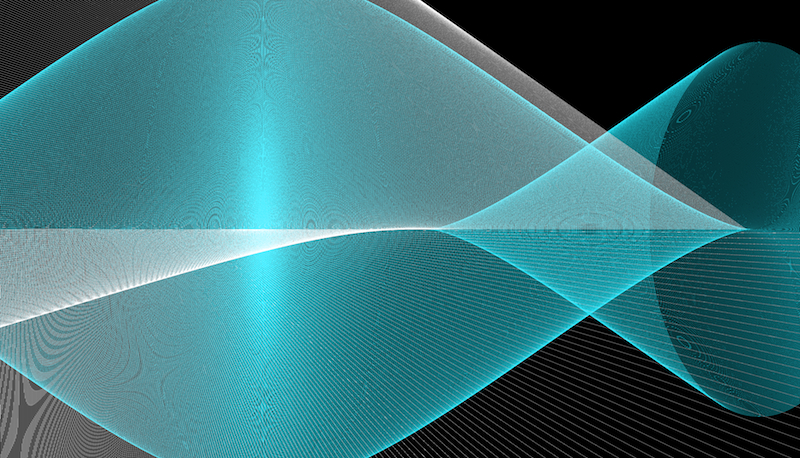
\includegraphics[width=0.9\textwidth]{img/binmatu}
	\caption{One of the Binmatu visuals}
	\label{fig:binmatu}
\end{figure}

From technical point of view, I am mainly using trigonometric functions for their rhythm and organic quality. These are fed with variables which are growing over the period of the whole piece, thus resulting in certain form of repetitive behavior when fed to e. g.\ sine function and linear narrative when used as direct controls of the attributes. Use of color is rather minimalistic, there is rarely more than 2 or 3 colors present.

After set of performances in Belgium, Czech Republic, Poland and Slovakia I was asked to create a new set for performing at NEXT festival in Slovakia. I have composed 9 new works and 9 new visuals in similar manner as the previous ones. There appeared a slight shift towards other psychoacoustic effects, from binaural beats (as in first works) towards Haas effect and other space illusions.

One particular composition is based around time delayed pulses, where the length of the delay is gradually shifted over the time by small steps. I have achieved this with setting up two separate pulses (one in each channel), with slight difference in frequency. I have calculated the difference in a way, that the pulses come to the temporary synchronization every 4 minutes (which is constant length of my works in this project). Use of pulses brings another spatial effect, and that being impulse response of the space. Frequency of the pulses gives sufficient time (142 milliseconds) for revealing the natural resonances and reverberations of the space. One can also perceive compression algorithm of the ear, which brings (in audio engineering slang, ``pumps'') these effects up between each pulse.

\subsection{Selected performances and installations} In this section, I would like to describe and evaluate some of Binmatu performances and installations. From performances, I have selected two most recent ones, quite different from each other providing ground for comparisons. First being performance in Studio Loos in The Hague during one of the \emph{Ephémère} evenings organized by Marie Guilleray. 

This event consisted from quite different performance, from experimental amateur vocal performances of graphical scores (Genetic choir \& Tanja Smit) to pop songs of Kathrin Grenzdörffer and her project \emph{Glanzkoffer}. Binmatu was scheduled last, which was from my experience a good decision. Unfortunately, by the time of the performance, big part of the audience left due to late hour. Since Loos offers quad-speaker setup, I decided to use it for my work by mapping front channels to rear in reverse. During my soundcheck I have prepared the speaker in traditional symmetric fashion, but over the night I noticed that listeners have chosen rather untraditional positions in the space, so I improvised and modified the directions of the rear speakers to cover sides of the small room rather than the center (which was already covered by front speakers). I was expecting a lot of interactions, comb filtering, reverb and other acousticians nightmares. Not being acoustician, I personally enjoy these effects very much and they have became an inspiration for further works and installations. 

As expected, sound was behaving oddly and quickly conquered the whole room. Judging from the point of a performer (partly out of the system), transients were completely lost in the reflections and reverb. Presence of the low frequencies was slightly lower, but as I said, I was happy with all the imperfections and acoustic errors of the space, because they served my purposes well.

Second event mentioned, contrasting to small studio performance, is \emph{Sonology Discussion Concert} presented in Arnold Schoenbergzaal of Royal Conservatory in The Hague. Arnold Schoenbergzall is spacious concert hall designed for larger events of various genres of music. For my years at Sonology, it has been a home to most of Sonology concerts. It was a special moment for me to finally present my work in such place and I treated it with adequate dignity.

\begin{figure}  
  \centering
    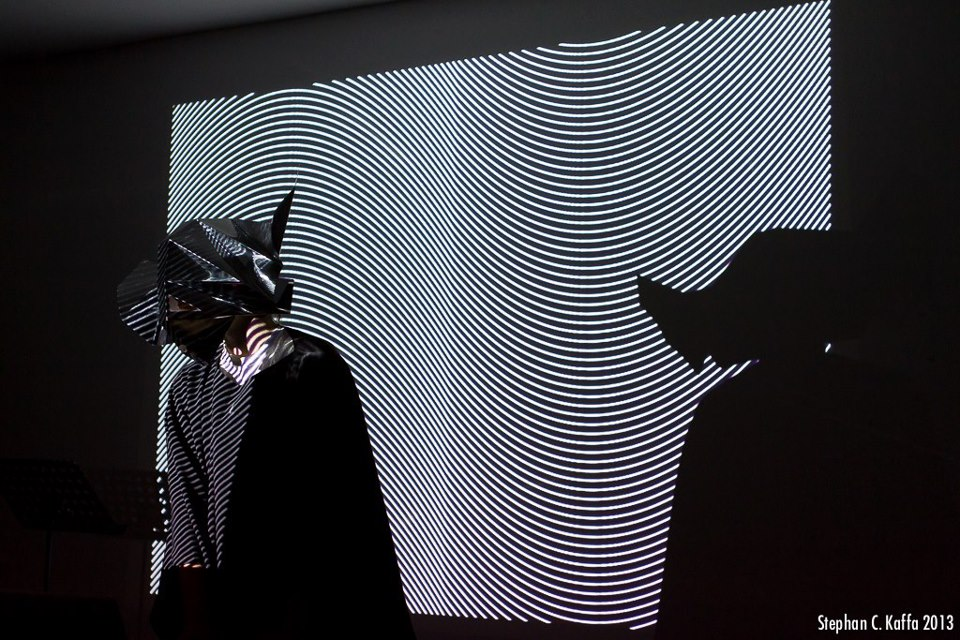
\includegraphics[width=0.9\textwidth]{img/binmatu_perfo}
	\caption{Binmatu performance in Studio Loos}
	\label{fig:binmatu_perfo}
\end{figure}

I have once again benefited from quad-speaker setup, and this time the order of rear speakers was not reversed. It has been quite successful in its realization. There were some minor disturbances with distortion of the speakers / mixing console at few points, but in the end I was satisfied with results. Hall provided sufficient ground for the grandiosity of certain pieces and previously described ``impulse'' piece had enormous impact because of the natural reverberation, which haven't smothered transients, yet allowed blossoming of impulse responses.

\subsection{Conclusion} Binmatu is still ongoing project. Over the course of year and a half, it has developed from uncertain coasts of self-searching vocal performance to clean and direct \emph{digitalism}. I still see myself with lack of expertise in performative aspect of the performance. I feel I need to research more art works dealing with ``musical spirituality'', ways of reaching deep into human mind, further than simple emotions, through medium of sound. After one of the performances, one composer studying classical composition in Bratislava, Slovakia came to me and said that he had very strange experience. He told me, that he has ``been places and remembered things which he believed were long forgotten''. I view it as beautiful compliment, especially, because at that point I knew I am not alone who perceives the psyche-delic (I choose to divide this word to embrace its original meaning) energy stored within these simple sounds. Other compliment I want to point out was from a girl, which pronounced, that she was not able to focus on any music after my performance. It worked as some kind of special spell which simply didn't let her to concentrate and listen during the rest of festival. I found it quite beautiful, I was astonished that my pieces can reach such levels of impact. How far can I possibly reach?

For the future, I see myself starting to work with Binmatu installations as well. Effort to transform my performance into infinite streams of sound and visuals. Embracing the site-specificity --- use of the acoustic properties of spaces, illusions, use of present objects as speakers with use of tactile transducers.

\clearpage
\section{Phasolume} Phasolume is an audiovisual installation that I've authored in collaboration with Agnes Szelag.

\subsection{Introduction} In 2011 and 2012 I have done a student exchange at Academy of Music in Cracow. This visit has resulted in few different collaborations, and I especially started to collaborate with Agnes Szelag, which has been on a residency at same place. Agnes Szelag is a California based sound artist, performer and composer. After receiving her title from Mills College, she performed and presented her work on festivals around USA and Europe. She has also authored few audiovisual installations. 

At the beginning of the year, Szelag started a group called Krakow Active Ensamble, which connected various musicians from the conservatory into one unifying experience of free improvisation and graphical scores. For my part, I have been mostly using my own software programmed in Max, JONO. Ensemble have been performing on various occasions in galleries, electroacoustic events and open jam sessions.

In the beginning of 2012, Agnes and I have decided to prepare an installation together. We both have made some works in this field before, but our standpoints were rather different. My main skill is dealing with technical concepts and hers was more of a conceptual and esthetical level --- outlook on the work as a whole unit. 

\subsection{Working process} Our basic idea was to implement organic behavior, imitation of processes observed in nature using sound and light. We believe, that such methods, when used correctly, can relate to some specific parts of our aesthetic appreciation. At the beginning, we wanted to place our installation permanently in some abandoned building. After some research and brainstorming, we have changed the plan to create and present installation directly in my apartment. Since I had one extra room which could have been used exactly for this purpose, it became an ideal environment. It is not very often that one has opportunity to work on installation not limited by time or gallery factors.

By the end of March, we have slowly started to grasp an idea for specifics of the project. We decided to focus on Fireflies (\emph{Lampyris noctiluca}) and their rhythmic and synchronizing behavior. We didn't wanted to make exact simulation, it was meant to relate to a feeling, or an atmosphere of the situation. For this purpose, I have developed little electronic insects --- robots, built from LEDs and vibration motors. Vibration motors were hand-picked from broken cellphones our friends donated to us. 

The part of main technical concept became to insert these (in the end 10) little robots into various jars in a way, that they hit the glass with their bodies when turned on. This resulted in very cricket-like sound, since the vibration motors behave a little like wings of an insect, especially when turned on in short (one or two second) bursts. This triggered our inspiration and we have started to create various sequences with computer and Arduino board. Using a sequencing patch I specially made for this purpose, we have been able to work with these robots as with any other MIDI instrument.

\begin{figure}  
  \centering
    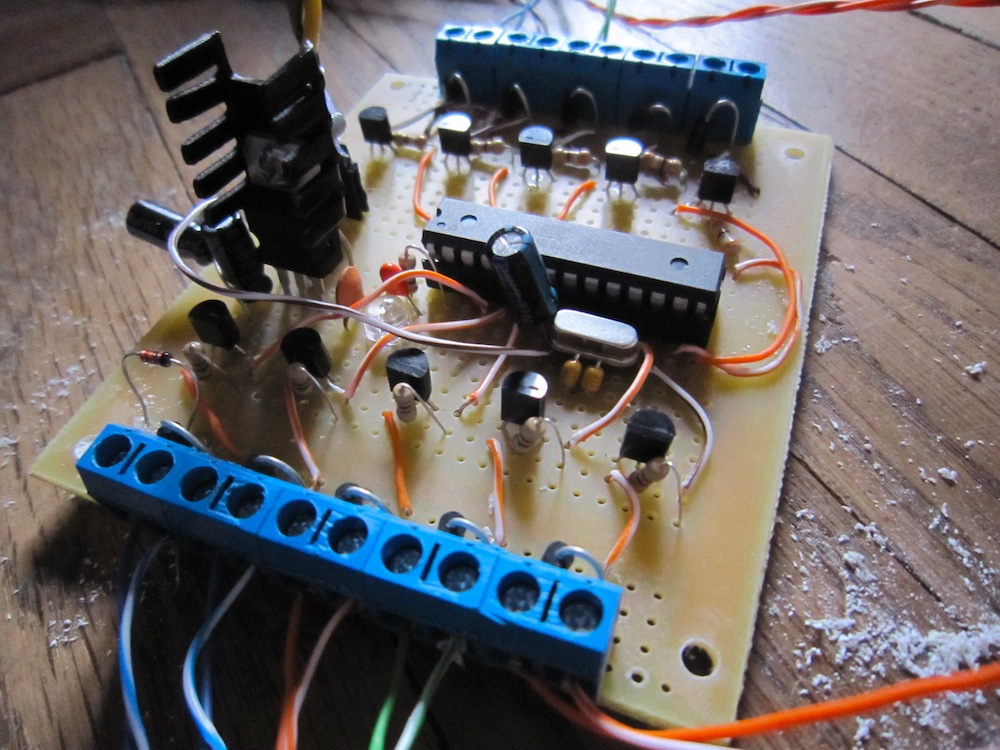
\includegraphics[width=0.9\textwidth]{img/phasolume}
	\caption{Custom designed circuit for Phasolume}
	\label{fig:phasolume}
\end{figure}

Last technical detail is, that in the end, the whole system was running without a normal computer, but from a circuit I have designed specifically for this process (see ~\ref{fig:phasolume}). This made it possible to make the whole core of the installation very small, transportable and easy to operate.

\subsection{Concept and execution} After the more technical part was finished, we started to focus more on the sequencing and general aesthetics of the installation. This has ended up in decision leaving preprogrammed (or precomposed) sequences and thinking more in a level of a generative algorithm. 

First algorithm idea was to create set of metronomes controlling the rhythm of robots, similarly to Ligeti's \emph{Poème symphonique}. One metronome per robot, each metronome with slightly higher (increments were equal) tempo than previous, e. g.\ there could be one with tempo of 60, other with 64, next one with 68 and so on. We wanted to create something which would start in sync, than slowly disperse in variations and come back to a sync afterwards. After I did the calculations, it turned out to be impossible if we wanted to keep slow-sync start and reasonable time of the whole cycle (from sync to sync). According to my calculations it was coming to length from tens of hours to hundreds of days. No visitor would be able to possibly perceive it, so we decided to create artificial resets --- resynchronizations. During resynchronization, new set of tempos is picked from the database and the whole sequence starts again.

The whole installation was set up, as mentioned, in my apartment. Core of the system was installed at the ceiling instead of a lamp. I have replaced the lamp with electricity socket, so it was possible to turn on the whole installation just by flicking of the regular light switch.

\subsection{Exhibition} After successful exhibition at my apartment (and slight problems with the police), we have been invited to present the installation at Krakers. Krakers is a yearly event happening in Cracow, dedicated to presenting little art collectives and mostly home galleries. We have setup the installation in another apartment and all together it was visited by more than 250 people. Many people have stayed with the installation for longer periods of time, simply enjoying the patterns emerging from the desynchronicity of this metronomic behavior.

\subsection{Conclusion} I really enjoyed this form of work, as well as collaboration with other artist. Especially an artist which comes from very different realities and contexts. I believe it resulted in fruitful combination of technical and aesthetic world and helped me with my own personal attitude towards creating public works of this kind.

\clearpage
\section{Site specific resonances}
\subsection{Introduction}
Site specific resonances was my latest project during the period of writing of this thesis. It was a sound installation setup in Vrije Academie Gemak in The Hague.

The project had started by my proposal to the gallery for creating site-specific sound installation. My aim was to do research on few topics, close to my aesthetical views --- minimalism, hidden technology and reusing / repurposing of materials. It ended up in creating set of performances more than installation, which I will explain in the end of the section.

I see the installation as somewhat continuation of my Binmatu project, where I am focusing on drones and subtle psychoacoustical effects hidden in the compositions. For this purposes, I have decided to work with resonant frequencies of the space. I have measured the room properties with measurement microphone and impulse response, than I extracted the most resonant frequencies and started composing.

\subsection{Technical aspects}

But before that, it is important to mention, that I have decided (as part of the minimalistic aesthetics) not to use regular speakers. I see them as somehow distracting elements. And, the method I have used instead --- tactile transducers --- worked much better visually, and sonically.

Tactile transducers are basically moving coils (like ones in the speaker), but without the speaker cone. They can be attached to any object, which has at least a bit moving body, and than they can use it as a cone. In a result, the object becomes a speaker. 

This of course brings many interesting aspects to the speaker. Mainly, it is inheriting the acoustic imperfections of the object. E.g.\ metallic plate resonates at certain frequencies and presents a long reverb (such as in plate reverb). I have, of course, exercised this greatly in my project.

Firstly, I have acquired various interesting objects which were laying around in the workshop of the gallery --- two metallic plates and one empty oil barrel. Than I created three different `stages' --- three different sound emitting objects. Two of those were connected to one amplifier and than to my computer, and one stage was totally separate from the main computer. To achieve this visual separation --- no cables running through the space\footnote{I believe there is important visual aspect to that. Element of surprise, perception of the object as truly autonomous sound emitting unit.} I have used few different technologies I had on hand. Sound was generated from microcomputer Raspberry Pi running sound programming language Chuck. This audio was than fed to small amplifier and finally to the object (to the transducer connected to it).

This solution gave me opportunity to have full control over what was happening in the room sound wise without need for jungle of wires and multichannel sound cards. It became especially important, when my worked in the gallery became more focused on performing with the installation rather than creating an standalone self-sustaining installation.

Visually, the installation was very minimalistic --- bare metallic plates emitting sound and one rambling oil can shaking in fearful drone. I personally find something very intriguing about simple metallic objects in space, especially when standing in space on their own, simple and raw in their full glory. They are like simple and understandable statements in a book yet they offer few different viewpoints.

\subsection{Performances}

I have performed with the installation 5 times, for various groups of people. First performances were happening during Hoogtij event, which turned out to be unfortunate. The crowds and delicate sound installations simply do not come together as a good match and I had ask people to be quite many times to make my work audible. Luckily the last three performances after unsuccessful two went quite successfully, one even having a very positive review at local art blog\footnote{\url{http://jegensentevens.nl/2013/03/de-frequentie-van-materiaal/}}.

\begin{figure}  
  \centering
    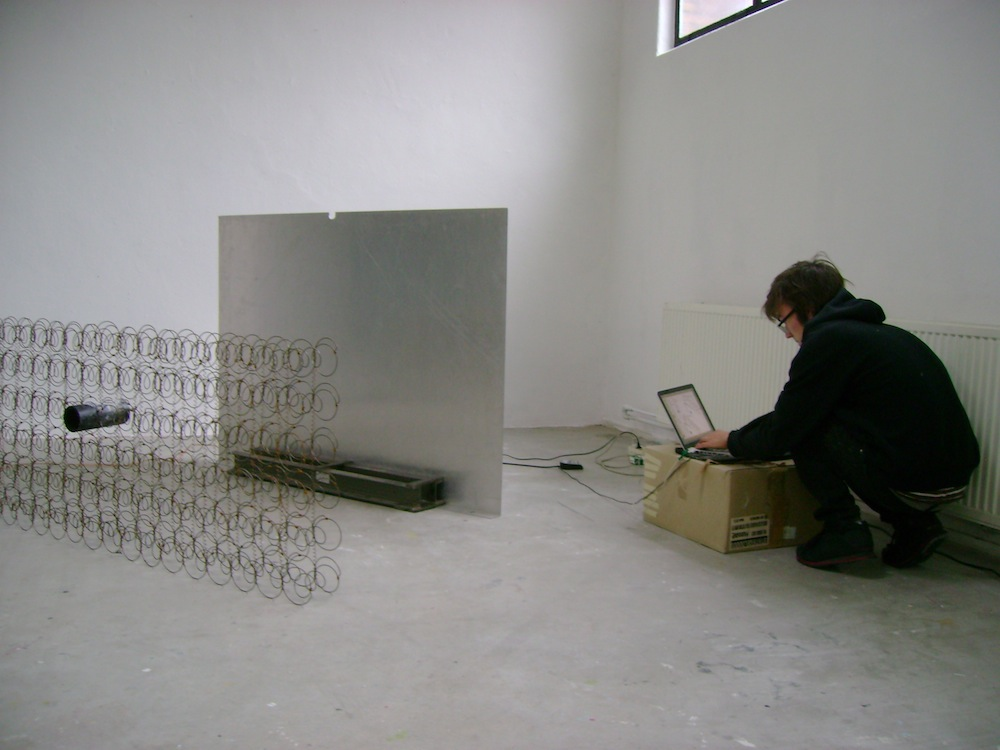
\includegraphics[width=0.9\textwidth]{img/sitespec}
	\caption{Site specific resonances performance}
	\label{fig:sitespec}
\end{figure}

Clear message from these works is to prepare the audience as much as possible for what is being presented, otherwise the subtle details which I base my work on go unnoticed, unexperienced --- thus worthless. It gave me a lot of inspiration for further projects, and I have been asked by the director of the gallery to come again to create something new for their spaces.

I have actually quite enjoyed the concept of creating installation as a system for performance, performing on non traditional setups sets beautiful atmosphere to the work and creates very different listening situation from the one we all know. 


\chapter{Conclusion}

\appendix
\chapter{List of selected performances, exhibitions, workshops and lectures}
\singlespacing

\textbf{2011}
\begin{itemize}
\item Participating in workshop of Seijiro Murayama and performing in A4, Bratislava
\item Exhibiting finnish version of interactive poem Basen at Live Herring 2011 festival in Finland
\item Solo exhibition - interactive installation about 4 modes of listening at Royal Conservatory, Den Haag
\item Leading 4-day workshop on untraditional ways of city sonification, Brno, Czech Republic
\item Leading workshop on Pure Data, audio programming and Processing and performing on Intermedia festival in Banská Bystrica, Slovakia
\item Performing on AudioArt festival, Cracow, Poland. Exhibiting live sound installation Sonodump, Krakow, Poland
\item Performing on NEXT festival, Bratislava Slovakia
\end{itemize}
\vspace{1cm}

\textbf{2012}
\begin{itemize}
\item Performing with Krakow Active Ensamble in Alchemia, Krakow, Poland
\item BINMATU performance on Progressbar birthday party, Bratislava, Slovakia
\item Artistic residency at OKNO, Brussels, Belgium
\item Performing at OEN, Krakow, Poland
\item Artistic presentation and performance at Multiplace festival, Brno, Czech Republic
\item BINMATU performance in Academy of Music, Krakow, Poland
\item OSMOGAS exhibition at TIK festival, Brussels, Belgium
\item OSMOGAS exhibition at Open House festival, Brussels, Belgium
\item BINMATU performance at TIK festival, Brussels, Belgium
\item BINMATU performance at Queerowy maj, Krakow, Poland
\item Performing with Krakow Active Ensamble in Alchemia, Krakow, Poland
\item Performing with Krakow Active Ensamble at Index errorum dzieciorum installation opening, Krakow, Poland
\item Phasolume installation with Agnes Szelag, Krakow, Poland
\item BINMATU performance at Dietla 449, Krakow, Poland
\item BINMATU performance at Slovak Radio, Bratislava, Slovakia
\item Leading workshop on digital audio, Pure Data and programming at Young composers festival, Bratislava, Slovakia
\item BINMATU performance at NK, Bratislava, Slovakia
\item BINMATU performance at Day of Sound, Bunkier Sztuki, Krakow, Poland
\item Performing at Haguestock, Den Haag, Netherlands
\item Performing with Luke Deane and Eugene Kim, Den Haag, Netherlands
\item BINMATU performance at NEXT festival, Slovakia
\end{itemize}
\vspace{1cm}

\textbf{2013}
\begin{itemize}
\item BINMATU performance at Ephemere, Den Haag, Netherlands
\item Performing at Art's Birthday, Brussels, Belgium
\item BINMATU performance at Institute of Sonology, Den Haag, Netherlands
\item Performing at Haguestock, Den Haag, Netherlands
\item Performing at LOM label showcase, Bratislava, Slovakia
\item Performing at Kraak festival, Aalst, Belgium
\item Performing with Bolka, Den Haag, Netherlands
\item Performing in Gemak gallery, Den Haag, Netherlands
\end{itemize}

\chapter{List of links to my projects}
\singlespacing
\begin{itemize}
\item My personal website \\ \url{http://mrkva.ovecka.be}
\item Binmatu website \\ \url{http://binmatu.net}
\item LOM (label I have founded) website \\ \url{http://zvukolom.org}
\item Phasolume project \\ \url{http://mrkva.ovecka.be/index.php?/interactive/phasolume-11/}
\item AudioArt ("Sonodump") performance \\ \url {https://vimeo.com/33858336}
\end{itemize}
\onehalfspacing

\bibliographystyle{apacite} 
\bibliography{general}
%\printbibliography

\end{document} 
